% $Id: template.tex 11 2007-04-03 22:25:53Z jpeltier $

\documentclass{vgtc}                          % final (conference style)
%\documentclass[review]{vgtc}                 % review
%\documentclass[widereview]{vgtc}             % wide-spaced review
%\documentclass[preprint]{vgtc}               % preprint
%\documentclass[electronic]{vgtc}             % electronic version

%% Uncomment one of the lines above depending on where your paper is
%% in the conference process. ``review'' and ``widereview'' are for review
%% submission, ``preprint'' is for pre-publication, and the final version
%% doesn't use a specific qualifier. Further, ``electronic'' includes
%% hyperreferences for more convenient online viewing.

%% Please use one of the ``review'' options in combination with the
%% assigned online id (see below) ONLY if your paper uses a double blind
%% review process. Some conferences, like IEEE Vis and InfoVis, have NOT
%% in the past.

%% Figures should be in CMYK or Grey scale format, otherwise, colour 
%% shifting may occur during the printing process.

%% These few lines make a distinction between latex and pdflatex calls and they
%% bring in essential packages for graphics and font handling.
%% Note that due to the \DeclareGraphicsExtensions{} call it is no longer necessary
%% to provide the the path and extension of a graphics file:
%% \includegraphics{diamondrule} is completely sufficient.
%%
\ifpdf%                                % if we use pdflatex
  \pdfoutput=1\relax                   % create PDFs from pdfLaTeX
  \pdfcompresslevel=9                  % PDF Compression
  \pdfoptionpdfminorversion=7          % create PDF 1.7
  \ExecuteOptions{pdftex}
  \usepackage{graphicx}                % allow us to embed graphics files
  \DeclareGraphicsExtensions{.pdf,.png,.jpg,.jpeg} % for pdflatex we expect .pdf, .png, or .jpg files
\else%                                 % else we use pure latex
  \ExecuteOptions{dvips}
  \usepackage{graphicx}                % allow us to embed graphics files
  \DeclareGraphicsExtensions{.eps}     % for pure latex we expect eps files
\fi%

%% it is recomended to use ``\autoref{sec:bla}'' instead of ``Fig.~\ref{sec:bla}''
\graphicspath{{figures/}{pictures/}{images/}{./}} % where to search for the images

\usepackage{microtype}                 % use micro-typography (slightly more compact, better to read)
\PassOptionsToPackage{warn}{textcomp}  % to address font issues with \textrightarrow
\usepackage{textcomp}                  % use better special symbols
\usepackage{mathptmx}                  % use matching math font
\usepackage{times}                     % we use Times as the main font
\renewcommand*\ttdefault{txtt}         % a nicer typewriter font
\usepackage{cite}                      % needed to automatically sort the references
\usepackage{tabu}                      % only used for the table example
\usepackage{booktabs}                  % only used for the table example
%% We encourage the use of mathptmx for consistent usage of times font
%% throughout the proceedings. However, if you encounter conflicts
%% with other math-related packages, you may want to disable it.


%% If you are submitting a paper to a conference for review with a double
%% blind reviewing process, please replace the value ``0'' below with your
%% OnlineID. Otherwise, you may safely leave it at ``0''.
\onlineid{0}

%% declare the category of your paper, only shown in review mode
\vgtccategory{Research}

%% allow for this line if you want the electronic option to work properly
\vgtcinsertpkg

%% In preprint mode you may define your own headline.
%\preprinttext{To appear in an IEEE VGTC sponsored conference.}

%% Paper title.

\title{Stock Price Analysis Visualization Tool}

%% This is how authors are specified in the conference style

%% Author and Affiliation (single author).
%%\author{Roy G. Biv\thanks{e-mail: roy.g.biv@aol.com}}
%%\affiliation{\scriptsize Allied Widgets Research}

%% Author and Affiliation (multiple authors with single affiliations).
%%\author{Roy G. Biv\thanks{e-mail: roy.g.biv@aol.com} %
%%\and Ed Grimley\thanks{e-mail:ed.grimley@aol.com} %
%%\and Martha Stewart\thanks{e-mail:martha.stewart@marthastewart.com}}
%%\affiliation{\scriptsize Martha Stewart Enterprises \\ Microsoft Research}

%% Author and Affiliation (multiple authors with multiple affiliations)
\author{Josiah Buxton\thanks{e-mail: josiah.buxton@colorado.edu}\\ %
 			\\ %
\and Christopher Godley\thanks{e-mail: christopher.godley@colorado.edu}\\ %
				 %
\and Brian Lubars \thanks{e-mail: brian.lubars@colorado.edu}\\ %
%
\and Kenneth Hunter Wapman \thanks{e-mail: kenneth.wapman@colorado.edu}\\ %
}
\affiliation{\scriptsize Computer Science Department \\ University of Colorado Boulder}

%% A teaser figure can be included as follows, but is not recommended since
%% the space is now taken up by a full width abstract.
%\teaser{
%  \includegraphics[width=1.5in]{sample.eps}
%  \caption{Lookit! Lookit!}
%}

%% Abstract section.
\abstract{The goal of this final project was to create a stock price analysis visualization tool that would aid individuals in making informed decisions about the stocks they buy and sell.  We created a webpage that informs a novice reader about stock price technical indicators in a narrative format.  It also allows the user to interact with two different visualizations.  One visualization introduces the technical indicators and demonstrates their relationships between each other.  The second visualization gives the user complete control in generating price and technical indicator graphs of a stock price dataset. 
} % end of abstract

%% ACM Computing Classification System (CCS). 
%% See <http://www.acm.org/about/class> for details.
%% We recommend the 2012 system <http://www.acm.org/about/class/class/2012>
%% For the 2012 system use the ``\CCScatTwelve'' which command takes four arguments.
%% The 1998 system <http://www.acm.org/about/class/class/2012> is still possible
%% For the 1998 system use the ``\CCScat'' which command takes four arguments.
%% In both cases the last two arguments (1998) or last three (2012) can be empty.

%\CCScatlist{
  %\CCScat{H.5.2}{User Interfaces}{User Interfaces}{Graphical user interfaces (GUI)}{};
  %\CCScat{H.5.m}{Information Interfaces and Presentation}{Miscellaneous}{}{}
%}

%% Copyright space is enabled by default as required by guidelines.
%% It is disabled by the 'review' option or via the following command:
% \nocopyrightspace

%%%%%%%%%%%%%%%%%%%%%%%%%%%%%%%%%%%%%%%%%%%%%%%%%%%%%%%%%%%%%%%%
%%%%%%%%%%%%%%%%%%%%%% START OF THE PAPER %%%%%%%%%%%%%%%%%%%%%%
%%%%%%%%%%%%%%%%%%%%%%%%%%%%%%%%%%%%%%%%%%%%%%%%%%%%%%%%%%%%%%%%%

\begin{document}

%% The ``\maketitle'' command must be the first command after the
%% ``\begin{document}'' command. It prepares and prints the title block.

%% the only exception to this rule is the \firstsection command
\firstsection{Introduction}

\maketitle

Stock trading can be very risky business when one is uneducated about the stocks he/she is buying.  Technical indicators have been made in the past to give traders an indication as to when a stock/how much will rise or fall.  Visualization tools have also been made, but many of them are inflexible and only contain a few technical analysis functions. The lack of a robust and extensive stock price data visualization tool is the motivation for this project.

Our goal was to provide a user interface that would allow a user to interact with a large set of stock price data and overlay different technical indicators on top of time series data.  We realized that if we were to employ all of these technical indicators, there would be a good chance that amateur and novice traders/analysts would be unfamiliar with the characteristics of these indicators.  In order to address this, we decided to expand the scope of our project to incorporate a learning experience where the user would scroll through a short lesson on each of the technical indicators before accessing our visualization tool.

\section{Related Work}
Stock data visualizations are a critical part of financial trading. Without interpretable
visualizations, a trader may miss a new trend as it forms when it would have been obvious with the right
tools. Yahoo is one of many sites out there that provide convenient and powerful stock tools. Without
the need of an account, anyone can go to finance.yahoo.com \cite{yahoo} and view relevant trading information
about any stock. This was the leading inspiration behind our visualization, as well as many others as we
discovered in our research. We wanted to duplicate the basic functionality of that site with our own spin
and organizational requirements. The foundation of this was the ability to display any stock’s value over
time in a consistent view. These views would be supplemented by the other functions we implemented
to analyze the trends.
There are many resources openly available online that discuss methods of how to best analyze
stock data. One of these that was extremely useful was the Technical Analysis from the University of
Cambridge \cite{tech}. This is a 183 page analysis of various stock indicators and trends. In this document, they
talk extensively about the various technical aspects of stock modeling, but they also show and discuss
many ways to visualize this data. In many ways, this was a great technical document to dive into, but
most of these methods simply generate various two-dimensional plots.
Some interesting multi-dimensional work has been done by Joseph and Indratmo in their paper
Visualizing Stock Market Data with Self-Organizing Map \cite{simuic}. Instead of the traditional two dimensional
scatterplots, they used an unsupervised learning algorithm to plot and group stocks onto a three
dimensional grid, where stocks are organized two dimensionally with the third dimension is proportional
to the company's market capitalization. The paper claims serious benefits from clustering stocks
together and treating stock clusters as individual nodes when making trading decisions. It’s an intriguing
look into the use of more than two dimensions for stock visualization, but ultimately they compared
their results to the Yahoo Finance as well, as it is truly such a robust tool. Due to this, we will try not to
include multi-dimensional visualizations in our work here.
From a user’s perspective, there may be reason to view stocks at an individual level or at a more
global level, however, where the general trend of the stock market is just as important. This is what the
self-organizing map from Joseph and Indratmo’s was aiming to do, but the paper from Simunic \cite{article}
shows that similar results can be found by simply using a heatmap and two dimensional space to reflect
the trends across all stocks plotted in that space. Each plot represents a grid in the overall visualization,
with zooming functionality for broad market views, or more specific stock trends. This was a much more
favorable style of visualization than the Joseph paper, but again they compared their results to the
functionality provided by the Yahoo Finance site, reiterating just how powerful and pervasive that
format is. Certain aspects from this visualization would be great to incorporate, however, as displaying
more than one stock at a time is a common need.

Even after more extensive research, we were left surprised with how good the Yahoo model
actually is, and therefore were not ashamed to emulate it as much as necessary to get the results we
desired. 
\section{Design Process}
\subsection{Data Wrangling}
We used the AlphaVantage API \cite{alpha} in order to obtain real-time stock data. We made queries to
capture data for six different stocks from the time of the stock’s inception. We captured the stocks’
price data through a time series daily adjusted module which returns the open, close, high, low, volume,
and adjusted close prices of an array of dates. We then used a variety of other modules to capture SMA,
EMA, STOCH, RSI, MACD technical indicators. We decided upon these indicators after researching commonly used analysis tools on investopedia.com \cite{invest}.  All of this data was stored into a python dictionary and then
outputted into json files. The json files are read in with javascript and displayed using D3.  We chose to work with D3 because we were very comfortable with making two dimensional plots out of loaded json data and as a programmer, you have a lot of control over particular aspects of the data.

\subsection{Visualization 1: Learning Tool}

\subsection{Visualization 2: Analysis Tool}
After our research, we knew that the most practical visualization tools used two dimensional scatter/line plots in order to plot time series data.  We decided to use both for all of the different data types we gathered. We wanted to give the user the ability to drill down to any type of technical indicator or price and plot a range of data from the dataset.  This is done by selecting categorical data in option boxes next to the visualization.  

There is also the option

\begin{figure}[h]
	\centering
	%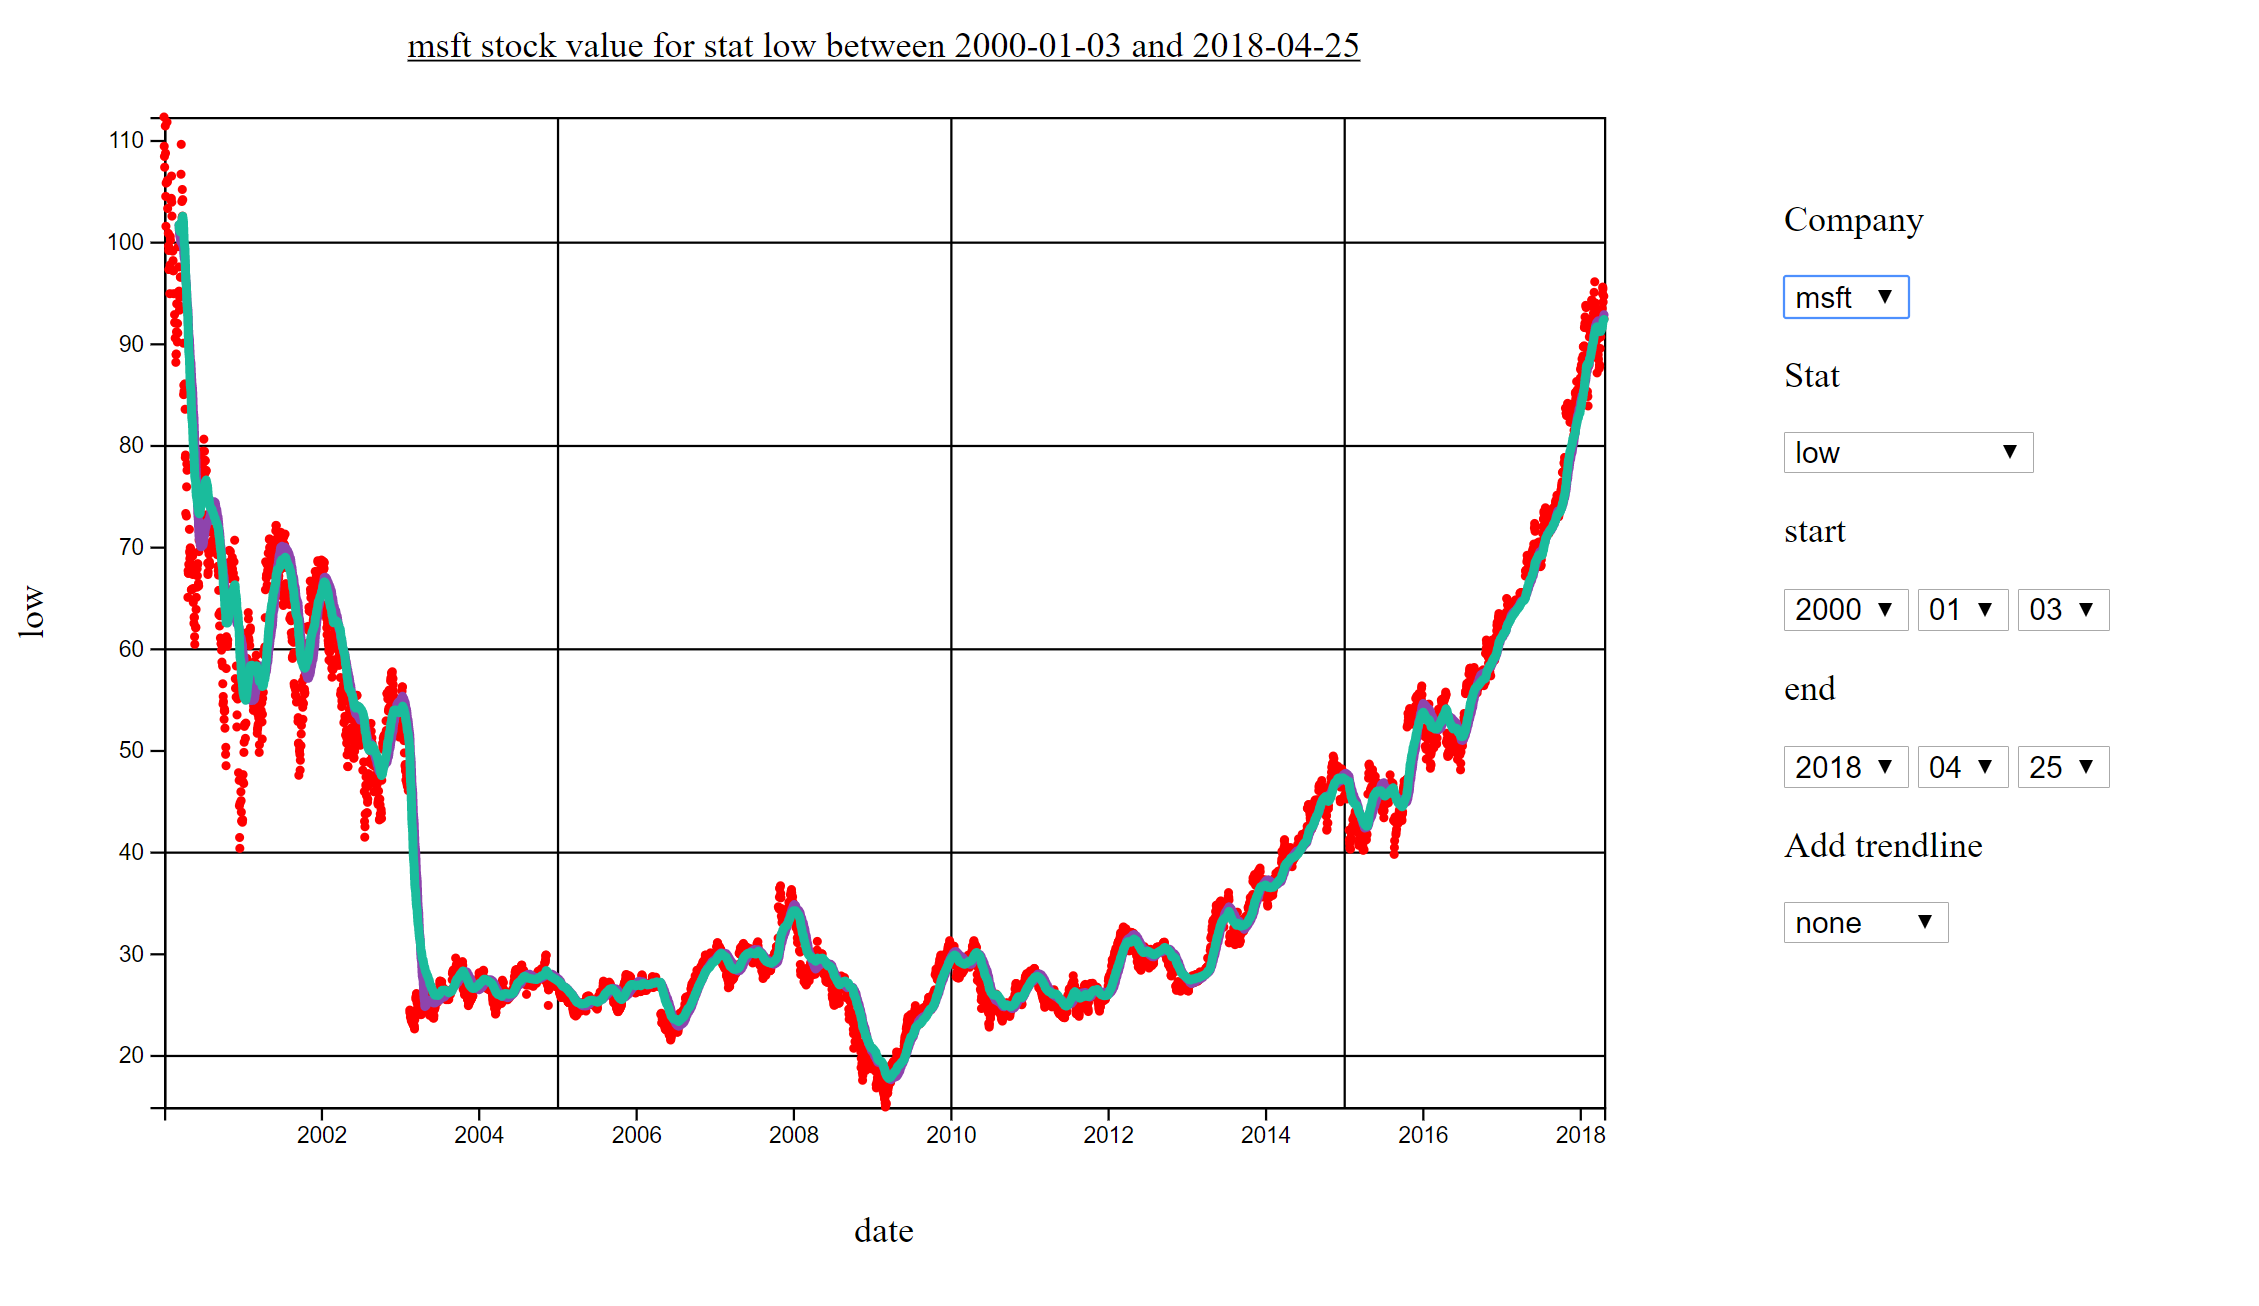
\includegraphics[scale=0.65]{vis2}
	%\caption{}
\end{figure}


\section{Discussion}


%\bibliographystyle{abbrv}
\bibliographystyle{abbrv-doi}
%\bibliographystyle{abbrv-doi-narrow}
%\bibliographystyle{abbrv-doi-hyperref}
%\bibliographystyle{abbrv-doi-hyperref-narrow}

\bibliography{template}
\end{document}
